\documentclass[12pt,letterpaper]{article}
\usepackage{graphicx,textcomp}
\usepackage{natbib}
\usepackage{setspace}
\usepackage{fullpage}
\usepackage{color}
\usepackage[reqno]{amsmath}
\usepackage{amsthm}
\usepackage{fancyvrb}
\usepackage{amssymb,enumerate}
\usepackage[all]{xy}
\usepackage{endnotes}
\usepackage{lscape}
\newtheorem{com}{Comment}
\usepackage{float}
\usepackage{hyperref}
\newtheorem{lem} {Lemma}
\newtheorem{prop}{Proposition}
\newtheorem{thm}{Theorem}
\newtheorem{defn}{Definition}
\newtheorem{cor}{Corollary}
\newtheorem{obs}{Observation}
\usepackage[compact]{titlesec}
\usepackage{dcolumn}
\usepackage{tikz}
\usetikzlibrary{arrows}
\usepackage{multirow}
\usepackage{xcolor}
\newcolumntype{.}{D{.}{.}{-1}}
\newcolumntype{d}[1]{D{.}{.}{#1}}
\definecolor{light-gray}{gray}{0.65}
\usepackage{url}
\usepackage{listings}
\usepackage{color}
\usepackage{parskip} 
\usepackage{subcaption}    % for subfigures

\definecolor{codegreen}{rgb}{0,0.6,0}
\definecolor{codegray}{rgb}{0.5,0.5,0.5}
\definecolor{codepurple}{rgb}{0.58,0,0.82}
\definecolor{backcolour}{rgb}{0.95,0.95,0.92}

\lstdefinestyle{mystyle}{
	backgroundcolor=\color{backcolour},   
	commentstyle=\color{codegreen},
	keywordstyle=\color{magenta},
	numberstyle=\tiny\color{codegray},
	stringstyle=\color{codepurple},
	basicstyle=\footnotesize,
	breakatwhitespace=false,         
	breaklines=true,                 
	captionpos=b,                    
	keepspaces=true,                 
	numbers=left,                    
	numbersep=5pt,                  
	showspaces=false,                
	showstringspaces=false,
	showtabs=false,                  
	tabsize=2
}
\lstset{style=mystyle}
\newcommand{\Sref}[1]{Section~\ref{#1}}
\newtheorem{hyp}{Hypothesis}

\title{Replication - Applied Stats II}
\date{Due: April 1, 2026}
\author{Sarah Magdihs}


\begin{document}
	\maketitle
	\textbf{\textit{Replicated Study:}} Schonfeld, B., \& Winter-Levy, S. (2021). Policy or Partisanship in the United Kingdom? Quasi-Experimental Evidence from Brexit. The Journal of Politics, 83(4), 1450–1461. https://doi.org/10.1086/712143
	\section{Introduction}
	This paper presents the replication for the final assignment. Specifically, I replicate and extend the study by Schonfeld and Winter-Levy (2021). First, I will provide the necessary context for understanding the original study, including the methodological approach and hypotheses. This is followed by the replication of all tables and figures in the chosen research paper. The replication will present the replicated outputs and discuss the inferences drawn from them by the original authors. Next, the paper will present the extensions - or \textit{"twists"} - that I have chosen to undertake.
	
	\section{Context: Original Study}
	According to Schonfeld and Winter-Levy (2021), a key question in political science scholarship continues to be whether voters are motivated by policy preferences or partisan identities. This question is by no means trivial, as its answer would have significant implications for theories of ideological responsiveness, political representation, and democratic accountability. In their study, the authors outline two main hypotheses that can be found in the literature: the ‘party-over-policy’ hypothesis and the ‘policy-over-party’ hypothesis. According to the ‘party-over-policy’ hypothesis, citizens lack coherent, stable ideological preferences. Instead, they respond to partisan cues when they evaluate policies and update their political views in order to match their political party. In contrast, the ‘policy-over-party’ hypothesis suggests that citizens actually have genuine policy preferences. Accordingly, these accounts understand party identity as "mostly endogenous to other political attitudes" (Schonfeld and Winter-Levy, 2021, p. 1451). 
	
	Despite decades of research, the extent to which these hypotheses hold remains contested, largely because providing definitive empirical evidence is methodologically challenging. In particular, disentangling the underlying mechanisms is rather difficult, as non-experimental research designs face endogeneity and selection problems, and ‘partisan intoxication’ and policy-motivation are often "observationally equivalent" (Schonfeld and Winter-Levy, 2021, p. 1451). One approach to overcome these challenges "is to study party realignments, which can occur when the policy position of a major party changes rapidly and significantly" (Schonfeld \& Winter-Levy, 2021, p. 1451). 
	
	Exploiting such a situation, the paper by Schonfeld and Winter-Levy (2021) focuses on the "sudden, unanticipated shift in Conservative Party positioning on Brexit following the surprising result of the 2016 referendum" as a case study. The British public voted to leave the European Union on June 23, 2016. As the outcome of the Referendum was uncertain, the authors contend that this interruption in the time series is quasi-exogenous. Furthermore, in the aftermath of the 2016 Brexit referendum in the UK, the British Conservative Party repositioned themselves as a pro-Brexit party, shifting its position in a matter of days. Furthermore, the British Election Study collected panel data immediately prior to and shortly after the referendum (Wave 8 and Wave 9).  
	
	Schonfeld and Winter-Levy (2021) primarily test two competing hypotheses. According to the Policy Voting Hypothesis, individuals’ pre-referendum Euroskepticism should predict subsequent changes in partisan identification. In contrast, the Partisan Intoxication Hypothesis predicts that supporters of the Conservative Party will adjust their Euroskepticism to align with the party’s new position. To examine the main hypotheses, the authors use an interrupted time series design. They compare respondents’ partisan identification and policy attitudes in Wave 8 (May 6-June 22, 2016) and Wave 9 (June 24-July 4, 2016) of the British Election Study.
	
	They find evidence that voters are indeed policy-motivated: Conservative partisans  "who were less Euroskeptic withdrew their support from the party following its sudden change in Brexit positioning, while more Euroskeptic voters, who previously had not affiliated as Conservatives, backed the newly Euroskeptic party" (Schonfeld \& Winter-Levy, 2021, p. 1451). Moreover, the show that this result is also reflected in their analyis on subsequent vote choice, finding that "Euroskeptics who did not vote Conservative in the 2015 election were substantially more likely to turn out for the Conservatives in 2017, while Conservative voters in 2015 who were not Euroskeptic were much less likely to vote Conservative in the election two years later" (Schonfeld \& Winter-Levy, 2021, p. 1451). While they also find some evidence that
	highlights the power of partisanship, "these shifts are small in comparison to the scale of party switching" (Schonfeld \& Winter-Levy, 2021, pp. 1451-1452). However, partisanship effects persist in other areas. Specifically, the authors found that "people who joined the Conservatives right after the referendum became more hostile to economic redistribution in the months to follow" (Schonfeld \& Winter-Levy, 2021, pp. 1452). Thus, the paper ultimately sheds light on the importance and merit of both hypotheses. 
	
	\section{Replication of the Original Study}
	The following subsections present the replicated tables and figures. I will briefly discuss the inferences the authors draw from these outputs. An overview of the findings has already been presented in section 2. 
	
	\subsection{Do voters change their partisan identification for policy reasons?}
	Schonfeld and Winter-Levy (2021) begin by testing the Policy Voting Hypothesis, which refers to the hypothesis that pre-referendum Euroskepticism predicts party-switching. Their first regression (Table 1) focuses on voters who identified as Conservatives before the referendum. 
	The response variable is a dummy variable that equals “1” if the respondent no longer identifies as a Conservative in Wave 9. The primary explanatory variable is pre-referendum Euroskepticism (continuous 0-10 scale). Higher values indicate higher Euroskepticism. Additionally, the model takes perceptions of changes in the Conservative Party’s level of Euroskepticism before and after the Referendum into account (and interacts this variable with Euroskepticism). 
	
	% Table created by stargazer v.5.2.3 by Marek Hlavac, Social Policy Institute. E-mail: marek.hlavac at gmail.com
	% Date and time: Wed, Apr 01, 2026 - 16:50:28
	\begin{table}[H] \centering 
		\caption{Euroskepticism and Defection from the Conservatives} 
		\label{} 
		\resizebox{0.9\textwidth}{!}{%
			\begin{tabular}{@{\extracolsep{5pt}}lccc} 
				\\[-1.8ex]\hline 
				\hline \\[-1.8ex] 
				& \multicolumn{3}{c}{\textit{Dependent variable: Defect from Conservatives}} \\ 
				\cline{2-4} 
				\\[-1.8ex] & \multicolumn{2}{c}{}
				\\[-1.8ex] & (1) & (2) & (3)\\ 
				\hline \\[-1.8ex] 
				Pre-Referendum Euroskepticism & $-$0.003$^{*}$ & $-$0.001 & 0.0001 \\ 
				& (0.001) & (0.001) & (0.001)  \\ 
				Perceived Change in Conservative Euroskepticism &  & 0.011$^{*}$ & 0.009$^{*}$ \\
				&  & (0.004) & (0.004) \\ 
				Age &  &  & $-$0.001$^{***}$ \\ 
				&  &  & (0.0002) \\ 
				Female &  &  & $-$0.007 \\ 
				&  &  & (0.007) \\ 
				White &  &  & $-$0.058$^{**}$ \\ 
				&  &  & (0.019) \\ 
				Scotland &  &  & 0.002 \\ 
				&  &  & (0.012) \\ 
				Wales &  &  & 0.021 \\ 
				&  &  & (0.014) \\ 
				Pre-referendum Euroskepticism:\\
				Perceived change in Conservative Euroskepticism &  & $-$0.001$^{*}$ & $-$0.001$^{*}$ \\ 
				&  & (0.001) & (0.001) \\ 
				Constant & 0.101$^{***}$ & 0.084$^{***}$ & 0.181$^{***}$ \\ 
				& (0.011) & (0.011) & (0.023) \\ 
				\hline \\[-1.8ex] 
				Observations & 7,330 & 6,476 & 6,216 \\ 
				R$^{2}$ & 0.001 & 0.001 & 0.006 \\ 
				Adjusted R$^{2}$ & 0.0004 & 0.001 & 0.005 \\ 
				Residual Std. Error & 0.272 (df = 7328) & 0.261 (df = 6472) & 0.258 (df = 6207) \\ 
				F Statistic & 3.912$^{*}$ (df = 1; 7328) & 2.709$^{*}$ (df = 3; 6472) & 4.554$^{***}$ (df = 8; 6207) \\ 
				\hline 
				\hline \\[-1.8ex] 
				\textit{Note:}  & \multicolumn{3}{r}{$^{*}$p$<$0.05; $^{**}$p$<$0.01; $^{***}$p$<$0.001} \\ 
			\end{tabular} 
		}
	\end{table} 
	
	The replication mirrors the original outputs in the research paper. Using OLS models, the analysis finds support for the Policy Voting Hypothesis. In their own words, "Euroskepticism negatively and significantly predicts leaving the Conservatives, the major party now most closely associated with Brexit" (Schonfeld \& Winter-Levy, 2021, p. 1454). Specifically, the first column indicates that a 1-point increase in pre-referendum Euroskepticism leads to a 0.3\% decrease in the probability of defection from the Conservatives. Moreover, the full model (column 3) shows that the interaction between pre-referendum Euroskepticism and perceptions of the party’s policy shift is significant. This means that “Conservatives who were less Euroskeptic and who perceived that the party had become increasingly Euroskeptic were especially likely to reject it” (Schonfeld \& Winter-Levy, 2021, p. 1454). While substantively modest, the effect is statistically significant.
	
	Next, Schonfeld and Winter-Levy (2021) test to what extent pre-referendum Euroskepticism predicts switching party identification from non-Conservative to Conservative following the Referendum. The response variable is a dummy variable that equals “1” if the respondent newly identifies as a Conservative in Wave 9. The primary explanatory variable is pre-referendum Euroskepticism (continuous 0-10 scale). Additionally, the model takes perceptions of changes in the Conservative Party’s level of Euroskepticism before and after the Referendum into account (and interacts this variable with Euroskepticism). 
	
	% Table created by stargazer v.5.2.3 by Marek Hlavac, Social Policy Institute. E-mail: marek.hlavac at gmail.com
	% Date and time: Wed, Apr 01, 2026 - 16:52:07
	\begin{table}[H] \centering 
		\caption{Euroskepticism and Joining the Conservatives} 
		\label{} 
		\resizebox{0.9\textwidth}{!}{%
			\begin{tabular}{@{\extracolsep{5pt}}lccc} 
				\\[-1.8ex]\hline 
				\hline \\[-1.8ex] 
				& \multicolumn{3}{c}{\textit{Dependent variable: Joined Conservatives}} \\ 
				\cline{2-4} 
				\\[-1.8ex] & \multicolumn{3}{c}{} 
				\\[-1.8ex] & (1) & (2) & (3)\\ 
				\hline \\[-1.8ex] 
				Pre-Referendum Euroskepticism & 0.007$^{***}$ & 0.007$^{***}$ & 0.006$^{***}$ \\ 
				& (0.0005) & (0.001) & (0.001) \\ 
				Perceived change in Conservative Euroskepticism &  & $-$0.003$^{*}$ & $-$0.004$^{**}$ \\ 
				&  & (0.001) & (0.001) \\ 
				Age &  &  & 0.0004$^{***}$ \\ 
				&  &  & (0.0001) \\ 
				Female &  &  & $-$0.002 \\ 
				&  &  & (0.003) \\ 
				White &  &  & $-$0.008 \\ 
				&  &  & (0.007) \\ 
				Scotland &  &  & $-$0.017$^{***}$ \\ 
				&  &  & (0.005) \\ 
				Wales &  &  & $-$0.012 \\ 
				&  &  & (0.006) \\ 
				Pre-referendum Euroskepticism:\\
				Perceived change in Conservative Euroskepticism &  & 0.001$^{***}$ & 0.001$^{***}$ \\ 
				&  & (0.0002) & (0.0002) \\ 
				Constant & $-$0.001 & 0.00004 & $-$0.007 \\ 
				& (0.003) & (0.004) & (0.009) \\ 
				\hline \\[-1.8ex] 
				Observations & 18,517 & 15,139 & 14,554 \\ 
				R$^{2}$ & 0.012 & 0.015 & 0.017 \\ 
				Adjusted R$^{2}$ & 0.012 & 0.015 & 0.017 \\ 
				Residual Std. Error & 0.198 (df = 18515) & 0.204 (df = 15135) & 0.202 (df = 14545) \\ 
				F Statistic & 216.857$^{***}$ (df = 1; 18515) & 78.431$^{***}$ (df = 3; 15135) & 31.854$^{***}$ (df = 8; 14545) \\ 
				\hline 
				\hline \\[-1.8ex] 
				\textit{Note:}  & \multicolumn{3}{r}{$^{*}$p$<$0.05; $^{**}$p$<$0.01; $^{***}$p$<$0.001} \\ 
			\end{tabular} 
		}
	\end{table} 
	
	Once again, the outputs of the replication are consistent with the results reported by Schonfeld and Winter-Levy (2021). The model shows that Euroskepticism predicts shifting support to the Conservatives. Specifically, the first column shows that 1-point increase in pre-referendum Euroskepticism generates a 0.7\% increase in the probability of switching to the Conservatives. Column 3 further suggest that Euroskeptic non-Conservatives who perceived an increase in the Conservative Party's Euroskepticism were especially likely to join the party. 
	
	\subsection{Do strong partisans change their policy preferences?}
	Following their test of the Policy Voting Hypothesis, the authors examine their second main hypothesis: the Partisan Intoxication Hypothesis. Concretely, they test whether pre-referendum Conservative Party identification predicts increasing Euroskepticism (post-Referendum). 
	
	Testing this hypothesis is particularly important since, as Schonfeld and Winter-Levy (2021) mention, some voters are more committed to their political party than others. In Figure 1, the authors show whether individuals with stron partisan ties to the Conservative Party were more
	likely to become Euroskeptic following the party's change in position. To do so, they split the data into three groups: strong Conservatives, moderate Conservatives, and non-Conservatives.The response variable is change in respondents’ Euroskepticism between Wave 8 and Wave 9. Furthermore, the main explanatory variables is perceived increase in Conservative Euroskepticism.
	
	\begin{figure}[H] 
		\centering
		
\includegraphics[width=0.8\textwidth]{figureone.png}  % adjust width as needed
		\caption{\small Perceived change in Conservative Euroskepticism \& change in personal Euroskepticism.}
		\label{fig:example}
	\end{figure}
	
	Once again, the replicated output is consistent with the original study. We can see here that "the intensity of Conservative partisanship determined the extent to which voters followed the party’s evolving position on the EU—or, more precisely, their perception of the party’s evolving position" (Schonfeld \& Winter-Levy, 2021, pp. 1456). This is further supported by the outputs of the regression analysis in Table 3. There is a positive, statistically singificant relationship between Conservative partisans’ perception of their party’s increasing Euroskepticism and their own Euroskepticism. Substantively, however, the effect seems rather small. For very strong Conservatives, a 1-unit increase in perceived Conservative Euroskepticism (measured on a 0-10 scale!) is associated with a 0.22-unit increase in personal Euroskepticism.
	
	% Table created by stargazer v.5.2.3 by Marek Hlavac, Social Policy Institute. E-mail: marek.hlavac at gmail.com
	% Date and time: Wed, Apr 01, 2026 - 17:17:16
	\begin{table}[H] \centering 
		\caption{Individual Shifts in Euroskepticism} 
		\label{} 
		\resizebox{0.9\textwidth}{!}{%
			\begin{tabular}{@{\extracolsep{5pt}}lcc} 
				\\[-1.8ex]\hline 
				\hline \\[-1.8ex] 
				& \multicolumn{2}{c}{\textit{Dependent variable:}} \\ 
				\cline{2-3} 
				\\[-1.8ex] & \multicolumn{2}{c}{} 
				\\[-1.8ex] & (1) & (2)\\ 
				\\[-1.8ex] & Moderate Conservatives & Very Strong
				Conservatives\\ 
				
				\hline \\[-1.8ex] 
				Perceived change in \\
				Conservative Euroskepticism & 0.139$^{***}$ & 0.220$^{***}$ \\ 
				& (0.011) & (0.020) \\ 
				Female & $-$0.055 & $-$0.109 \\ 
				& (0.054) & (0.113) \\ 
				Age & 0.006$^{***}$ & 0.004 \\ 
				& (0.002) & (0.004) \\ 
				White & 0.094 & $-$0.186 \\ 
				& (0.154) & (0.300) \\ 
				Scotland & 0.131 & 0.099 \\ 
				& (0.096) & (0.192) \\ 
				Wales & 0.017 & $-$0.324 \\ 
				& (0.111) & (0.245) \\ 
				Constant & $-$1.161$^{***}$ & $-$0.573 \\ 
				& (0.178) & (0.340) \\ 
				\hline \\[-1.8ex] 
				Observations & 5,000 & 1,180 \\ 
				R$^{2}$ & 0.038 & 0.101 \\ 
				Adjusted R$^{2}$ & 0.036 & 0.097 \\ 
				Residual Std. Error & 1.882 (df = 4993) & 1.883 (df = 1173) \\ 
				F Statistic & 32.559$^{***}$ (df = 6; 4993) & 22.025$^{***}$ (df = 6; 1173) \\ 
				\hline 
				\hline \\[-1.8ex] 
				\textit{Note:}  & \multicolumn{2}{r}{$^{*}$p$<$0.05; $^{**}$p$<$0.01; $^{***}$p$<$0.001} \\ 
			\end{tabular} 
		}
	\end{table} 
	
	\subsection{Do new Conservatives adopt right-wing attitudes toward redistribution?}
	Following this analysis, the authors examine whether new Conservatives adopt right-wing attitudes
	toward redistribution. This analysis is meant to show the broader effects of that changes in party affiliation may carry with them. If new partisans indeed update their policy preferences, this would provide evidence that partisanship can have an influence even among voters who have apparently switched parties due to perceived congruence on policy issues. 
	
	Concretely, Schonfeld and Winter-Levy (2021) posit that "if partisanship shapes the development of voters’ policy preferences, Conservative affiliation should reduce an individual’s support for redistribution, since the Conservatives are the major party most hostile to this approach to economic policy" (Schonfeld and Winter-Levy, 2021, p. 1456). To illustrate this argument, they show that the Conservative Party was perceived as the most anti-redistribution party in both
	wave 7 (pre-referendum) and wave 11 (post-referendum) (see Figure 2).
	
	\begin{figure}[H]
		\centering
		\begin{subfigure}[b]{0.48\textwidth}
			\centering
			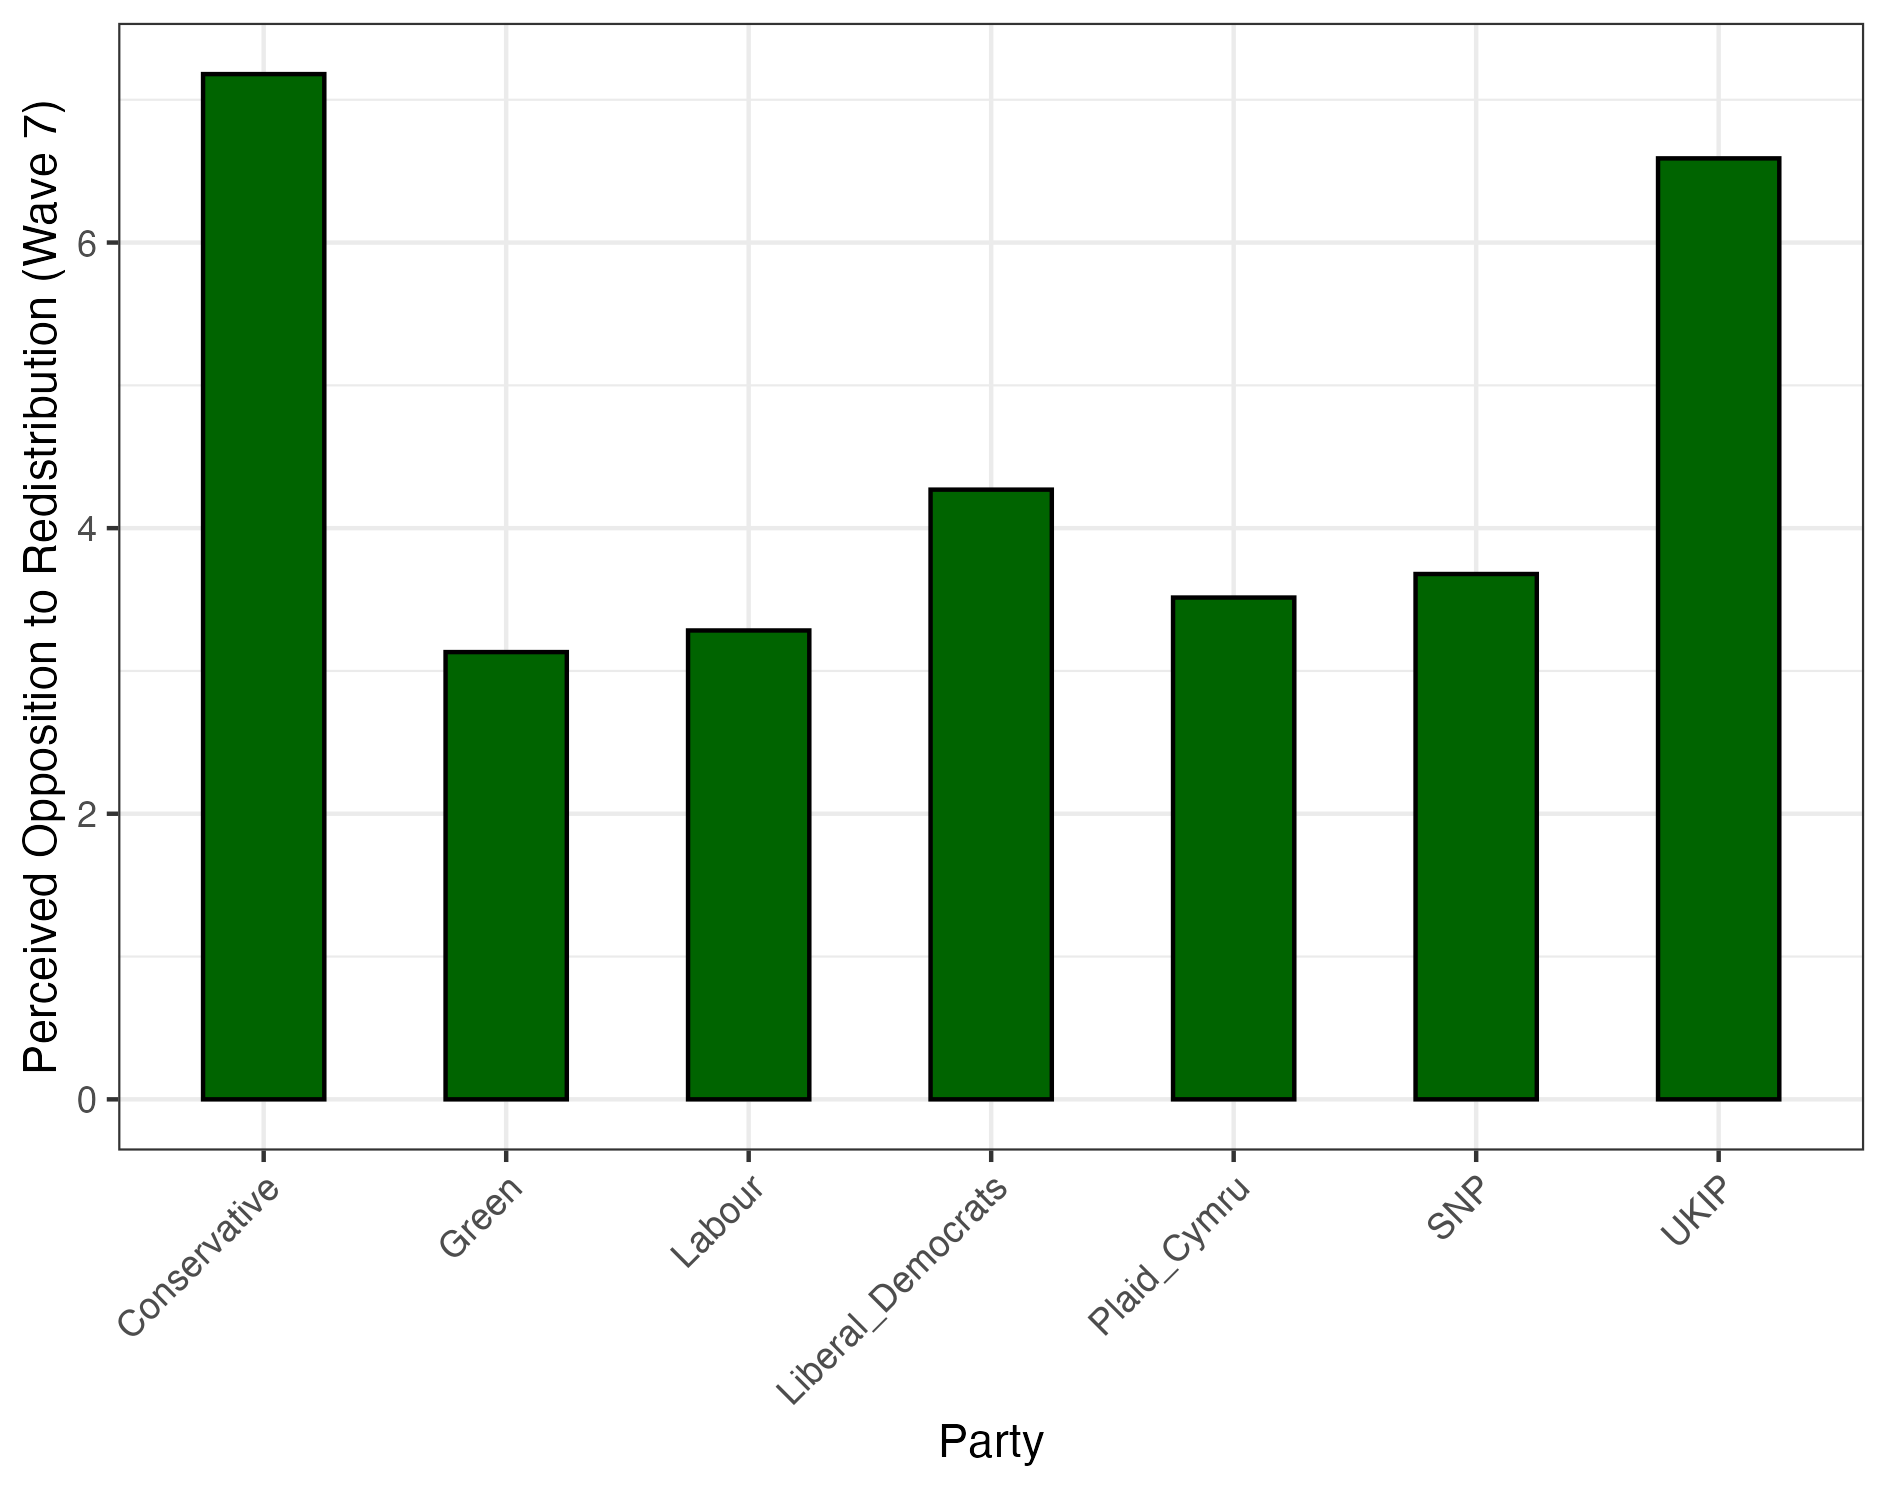
\includegraphics[width=\textwidth]{figure2_7.png}
			\caption{Wave 7}
			\label{fig:sub1}
		\end{subfigure}
		\hfill
		\begin{subfigure}[b]{0.48\textwidth}
			\centering
			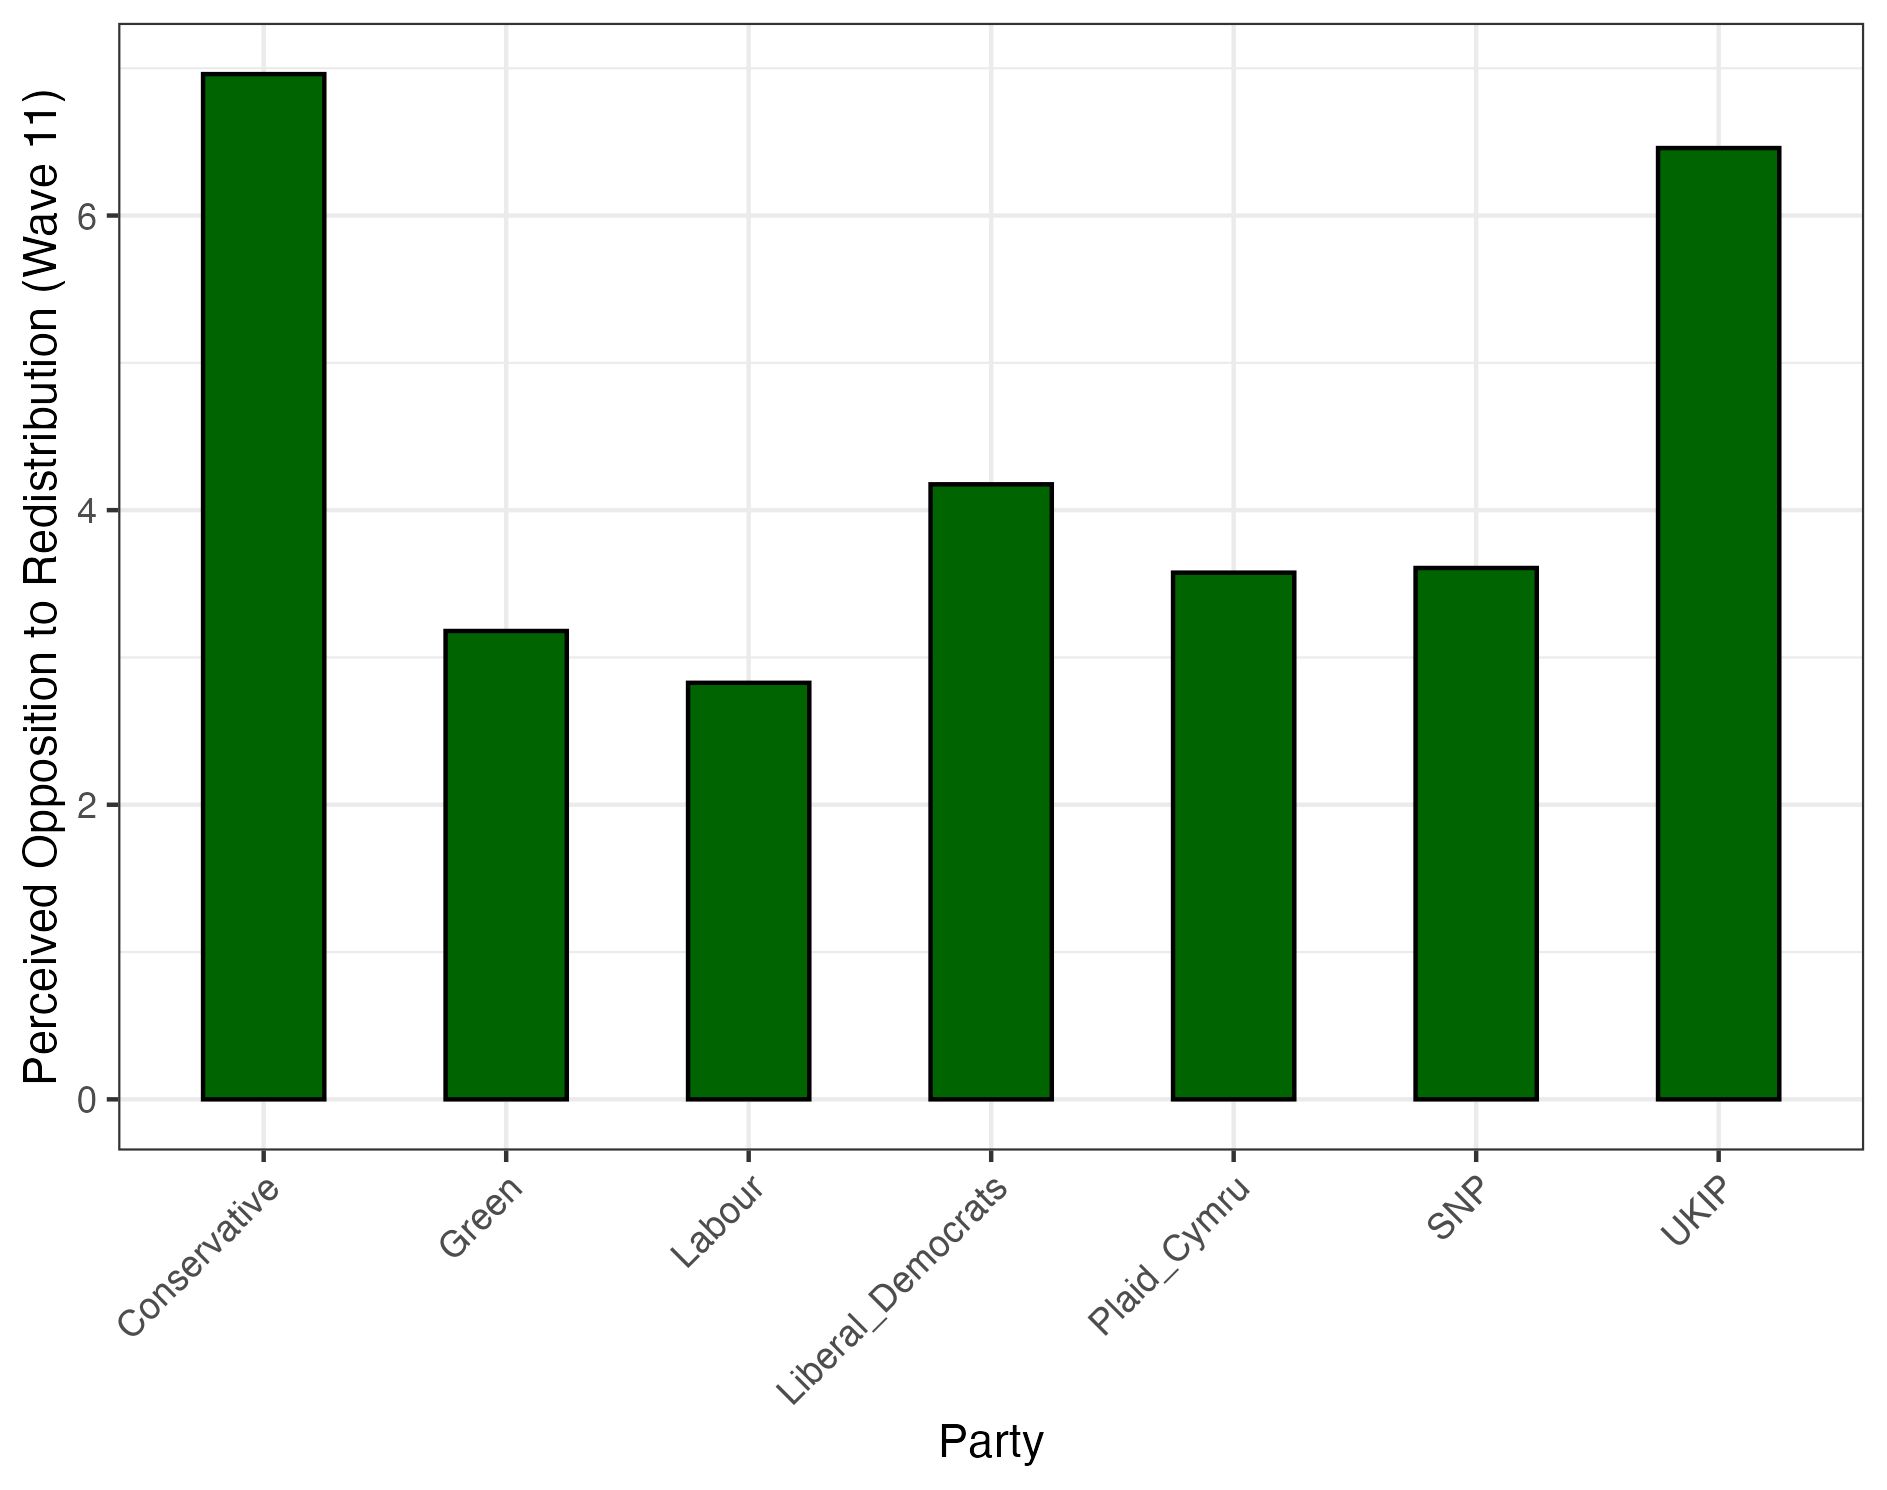
\includegraphics[width=\textwidth]{figure2_11.png}
			\caption{Wave 11}
			\label{fig:sub2}
		\end{subfigure}
		\caption{\small Perceived opposition to redistribution by party, waves 7 and 11; SNP = Scottish National Party; UKIP = UK Independence Party}
		\label{fig:figure2}
	\end{figure}
	
	For the regression analysis, the authors test the extent of the effect of joining the Conservatives on changes in attitudes toward redistribution. The response variable is Change in Opposition to Redistribution. This was measured by subtracting the level of opposition to redistribution in wave 7 of the BES (April 2016 and May 2016) from the level of opposition to redistribution in wave 11 (April 2017 and May 2017). These waves were chosen by the authors because they are the most recent post- and pre-referendum survey waves, respectively, that ask about redistribution preferences. 
	
	Table 4 presents the outputs from the OLS models. The authors find "a positive association between joining the Conservatives and increased opposition to redistribution" (Schonfeld and Winter-Levy, 2021, p. 1457). Specifically, column 1 shows that "affiliating with the Conservative Party is associated with more than a half-point increase in opposition to redistribution on a 10-point scale" (Schonfeld and Winter-Levy, 2021, p. 1457). Furthermore, column 2 and 3 show that the effect is stronger among the non-UKIP sample. Thus, the shift in economic attitudes towards more right-wing positions is more relevant for new partisans that were not previously associated with an anti-redistribution party. Once again, the replicated table mirrors the results from the original paper.
	
	\begin{table}[H] \centering 
		\caption{Joining the Conservatives and Opposition to Redistribution} 
		\label{tab:joiningconservatives} 
		\begin{tabular}{@{\extracolsep{3pt}}lccc} 
			\\[-1.8ex]\hline 
			\hline \\[-1.8ex] 
			& \multicolumn{3}{c}{\textit{Dependent variable: Change in Opposition to Redistribution}} \\ 
			\cline{2-4} 
			\\[-1.8ex] & Overall & Non-UKIP & UKIP \\ 
			\hline \\[-1.8ex] 
			Joined Conservatives & 0.542$^{***}$ & 0.605$^{***}$ & 0.042 \\ 
			& (0.133) & (0.158) & (0.285) \\ 
			White & 0.179 & 0.155 & 0.360 \\ 
			& (0.119) & (0.120) & (0.528) \\ 
			Age & $-$0.001 & $-$0.003 & 0.008 \\ 
			& (0.002) & (0.002) & (0.007) \\ 
			Female & $-$0.009 & 0.0001 & 0.003 \\ 
			& (0.052) & (0.054) & (0.191) \\ 
			Scotland & $-$0.162$^{*}$ & $-$0.109 & $-$0.472 \\ 
			& (0.071) & (0.071) & (0.468) \\ 
			Wales & $-$0.051 & $-$0.112 & 0.536 \\ 
			& (0.091) & (0.094) & (0.312) \\ 
			Constant & $-$0.161 & $-$0.094 & $-$0.518 \\ 
			& (0.144) & (0.146) & (0.631) \\ 
			\hline \\[-1.8ex] 
			Observations & 9,065 & 8,086 & 979 \\ 
			R$^{2}$ & 0.003 & 0.003 & 0.007 \\ 
			Adjusted R$^{2}$ & 0.002 & 0.002 & 0.001 \\ 
			Residual Std. Error & 2.477 (df = 9058) & 2.415 (df = 8079) & 2.906 (df = 972) \\ 
			F Statistic & 4.155$^{***}$ (df = 6; 9058) & 3.804$^{***}$ (df = 6; 8079) & 1.090 (df = 6; 972) \\ 
			\hline 
			\hline \\[-1.8ex] 
			\textit{Note:}  & \multicolumn{3}{r}{UKIP = UK Independence Party; $^{*}$p$<$0.05; $^{**}$p$<$0.01; $^{***}$p$<$0.001} \\ 
		\end{tabular} 
	\end{table} 
	
	\subsection{Has changing partisanship influenced actual voting?}
	Lastly, the authors examine whether these shifts in partisanship have potentially had long-term effects. To do so, they test whether the change in Conservative positioning on Brexit has influenced voting behavior and electoral outcomes. However, this analysis cannot make causal claims. To examine the relationship between Euroskepticism and voting in the 2015 and 2017 elections, the authors use data from wave 6 (May 2015, after the 2015 election) and wave 13 (June 2017, 2017 election) of the BES.
	
	Table 5 presents the analysis for individuals who reported voting for the Conservatives in the 2015 election. The authors find that there is a "consistent negative relationship between 2015 Euroskepticism and the likelihood of defecting from the (now more Euroskeptic) Conservatives in 2017. The effects are substantively large: a one-unit increase in Euroskepticism on the 10-point scale (in 2015) makes someone 2.9\% less likely to abandon the Conservatives in the 2017 election" (Schonfeld and Winter-Levy, 2021, p. 1459).
	
	\begin{table}[H] \centering
		\caption{Euroskepticism and Defecting from Conservatives} 
		\label{tab:euroskepticdefect} 
		\resizebox{\textwidth}{!}{%
			\begin{tabular}{@{\extracolsep{5pt}}lccc} 
				\\[-1.8ex]\hline 
				\hline \\[-1.8ex] 
				& \multicolumn{3}{c}{\textit{Dependent variable: Defected from Conservatives}} \\ 
				\cline{2-4} 
				\\[-1.8ex] & (1) & (2) & (3)\\ 
				\hline \\[-1.8ex] 
				2015 Euroskepticism & $-$0.029$^{***}$ & $-$0.031$^{***}$ & $-$0.026$^{***}$ \\ 
				& (0.003) & (0.003) & (0.003) \\ 
				Perceived change \\in Conservative Euroskepticism &  & 0.009 & 0.010 \\ 
				&  & (0.008) & (0.008) \\ 
				Age &  &  & $-$0.004$^{***}$ \\ 
				&  &  & (0.001) \\ 
				Female &  &  & 0.023 \\ 
				&  &  & (0.015) \\ 
				White &  &  & $-$0.020 \\ 
				&  &  & (0.041) \\ 
				Scotland &  &  & $-$0.053$^{*}$ \\ 
				&  &  & (0.026) \\ 
				Wales &  &  & 0.024 \\ 
				&  &  & (0.027) \\ 
				2015 Euroskepticism: Perceived \\change in Conservative Euroskepticism &  & $-$0.001 & $-$0.001 \\ 
				&  & (0.001) & (0.001) \\ 
				Constant & 0.358$^{***}$ & 0.362$^{***}$ & 0.608$^{***}$ \\ 
				& (0.023) & (0.028) & (0.053) \\ 
				\hline \\[-1.8ex] 
				Observations & 2,142 & 1,902 & 1,902 \\ 
				R$^{2}$ & 0.047 & 0.059 & 0.096 \\ 
				Adjusted R$^{2}$ & 0.047 & 0.058 & 0.092 \\ 
				Residual Std. Error & 0.332 (df = 2140) & 0.321 (df = 1898) & 0.315 (df = 1893) \\ 
				F Statistic & 105.620$^{***}$ (df = 1; 2140) & 39.927$^{***}$ (df = 3; 1898) & 25.150$^{***}$ (df = 8; 1893) \\ 
				\hline 
				\hline \\[-1.8ex] 
				\textit{Note:}  & \multicolumn{3}{r}{$^{*}$p$<$0.05; $^{**}$p$<$0.01; $^{***}$p$<$0.001} \\ 
			\end{tabular}%
		}
	\end{table}
	
	Table 6 presents the results for individuals who did not vote for the Conservatives in the 2015 election. In this case, the authors find "a clear positive relationship between their level of Euroskepticism in 2015 and the probability that they voted for the Conservatives in 2017. A one-unit increase in 2015 Euroskepticism (on the 10-point scale) makes a non-Conservative as much as 4.7\% more likely to vote for the Conservatives in 2017" (Schonfeld and Winter-Levy, 2021, p. 1459). Thus, the authors posit that the Conservative Party's change in policy position on Brexit has had effects beyond voters’ partisan identities and self-reported policy preferences.
	\begin{table}[H] \centering
		\caption{Euroskepticism and Switching Vote to Conservatives} 
		\label{tab:euroskepticswitch} 
		\resizebox{\textwidth}{!}{%
			\begin{tabular}{@{\extracolsep{5pt}}lccc} 
				\\[-1.8ex]\hline 
				\hline \\[-1.8ex] 
				& \multicolumn{3}{c}{\textit{Dependent variable: Switched to Conservatives}} \\ 
				\cline{2-4} 
				\\[-1.8ex] & (1) & (2) & (3)\\ 
				\hline \\[-1.8ex] 
				2015 Euroskepticism & 0.047$^{***}$ & 0.049$^{***}$ & 0.047$^{***}$ \\ 
				& (0.002) & (0.002) & (0.002) \\ 
				Perceived change \\in Conservative Euroskepticism &  & 0.005 & 0.004 \\ 
				&  & (0.004) & (0.004) \\ 
				Age &  &  & 0.002$^{***}$ \\ 
				&  &  & (0.0004) \\ 
				Female &  &  & $-$0.015 \\ 
				&  &  & (0.012) \\ 
				White &  &  & 0.061$^{*}$ \\ 
				&  &  & (0.028) \\ 
				Scotland &  &  & 0.010 \\ 
				&  &  & (0.015) \\ 
				Wales &  &  & $-$0.034 \\ 
				&  &  & (0.020) \\ 
				2015 Euroskepticism: Perceived \\change in Conservative Euroskepticism &  & 0.001$^{*}$ & 0.001$^{*}$ \\ 
				&  & (0.001) & (0.001) \\ 
				Constant & $-$0.068$^{***}$ & $-$0.076$^{***}$ & $-$0.228$^{***}$ \\ 
				& (0.011) & (0.012) & (0.035) \\ 
				\hline \\[-1.8ex] 
				Observations & 4,388 & 3,758 & 3,758 \\ 
				R$^{2}$ & 0.164 & 0.203 & 0.210 \\ 
				Adjusted R$^{2}$ & 0.164 & 0.202 & 0.208 \\ 
				Residual Std. Error & 0.367 (df = 4386) & 0.364 (df = 3754) & 0.363 (df = 3749) \\ 
				F Statistic & 861.685$^{***}$ (df = 1; 4386) & 318.651$^{***}$ (df = 3; 3754) & 124.664$^{***}$ (df = 8; 3749) \\ 
				\hline 
				\hline \\[-1.8ex] 
				\textit{Note:}  & \multicolumn{3}{r}{$^{*}$p$<$0.05; $^{**}$p$<$0.01; $^{***}$p$<$0.001} \\ 
			\end{tabular}%
		}
	\end{table}
	
	\section{Extension}
	Having replicated the original study, I will now move on to the extension. Following the suggestions listed in the instructions, I decided upon three extensions. Firstly, I essenitally performed a robustness check of the model by rerunning the full models in Table 1 and 2 using a logstic regression model. Secondly, I included an partisan strength as an additional control. Lastly, I tested whether the results change if we were to use an alternative measure for Euroskepticism. The extensions and their rationale will be discussed in more detail below. Please note that the extensions solely focus on the models presented in Table 1 and 2, which pertain to the question whether voters change their partisan identification for policy reasons. 
	
	\subsection{Logistic Models}
	Firstly, I decided to re-run the analyses from Section 3.1 using a logistic regression. The original study uses OLS models. However, the outcome variables are binary, which would suggest that a logistic model is more appropriate. I am assuming the authors chose OLS models due to the quasi-experimental setup. Thus, the results would be further strengthened if the logistic models show similar results. (However, coefficients cannot be compared 1:1 given that they are scaled differently).
	
	Table 7 and 8 present the results of logistic regressions alongside the original OLS models for the outcomes Defection from Conservatives and Joining Conservatives. While the coefficients themselves cannot be directly compared, the outputs show that the significance and direction of the effects remain the same.
	
	\begin{table}[H] \centering 
		\caption{Euroskepticism and Defection from the Conservatives: OLS vs Logistic} 
		\label{} 
		\resizebox{0.9\textwidth}{!}{%
			\begin{tabular}{@{\extracolsep{5pt}}lcc} 
				\\[-1.8ex]\hline 
				\hline \\[-1.8ex] 
				& \multicolumn{2}{c}{\textit{Dependent variable: Defect from Conservatives}} \\ 
				\cline{2-3} 
				\\[-1.8ex] & \textit{OLS} & \textit{Logistic} \\ 
				\\[-1.8ex] & (1) & (2)\\ 
				\hline \\[-1.8ex] 
				Pre-Referendum Euroskepticism & 0.0001 & 0.005 \\ 
				& (0.001) & (0.021) \\ 
				Perceived Change in Conservative Euroskepticism & 0.009$^{**}$ & 0.129$^{**}$ \\ 
				& (0.004) & (0.062) \\ 
				Age & $-$0.001$^{***}$ & $-$0.013$^{***}$ \\ 
				& (0.0002) & (0.003) \\ 
				Female & $-$0.007 & $-$0.109 \\ 
				& (0.007) & (0.101) \\ 
				White & $-$0.058$^{***}$ & $-$0.619$^{***}$ \\ 
				& (0.019) & (0.214) \\ 
				Scotland & 0.002 & 0.036 \\ 
				& (0.012) & (0.178) \\ 
				Wales & 0.021 & 0.292 \\ 
				& (0.014) & (0.192) \\ 
				Pre-referendum Euroskepticism: \\
				Perceived Change in Conservative Euroskepticism & $-$0.001$^{**}$ & $-$0.016$^{**}$ \\ 
				& (0.001) & (0.007) \\ 
				Constant & 0.181$^{***}$ & $-$1.260$^{***}$ \\ 
				& (0.023) & (0.293) \\ 
				\hline \\[-1.8ex] 
				Observations & 6,216 & 6,216 \\ 
				R$^{2}$ & 0.006 &  \\ 
				Adjusted R$^{2}$ & 0.005 &  \\ 
				Log Likelihood &  & $-$1,588.203 \\ 
				Akaike Inf. Crit. &  & 3,194.406 \\ 
				Residual Std. Error & 0.258 (df = 6207) &  \\ 
				F Statistic & 4.554$^{***}$ (df = 8; 6207) &  \\ 
				\hline 
				\hline \\[-1.8ex] 
				\textit{Note:}  & \multicolumn{2}{r}{$^{*}$p$<$0.1; $^{**}$p$<$0.05; $^{***}$p$<$0.01} \\ 
			\end{tabular} 
		}
	\end{table}
	
	As shown in Table 7, the analysis indicates that the perceived change in Conservative Euroskepticism is positively associated with defection in both OLS and logistic models. 
	The interaction between pre-referendum Euroskepticism and perceived change in Conservative Euroskepticism remains significant and negative in both models. This suggest that the results should be robust to model specifications. 
	
	\begin{table}[H] \centering 
		\caption{Euroskepticism and Joining to Conservatives: OLS vs Logistic} 
		\label{} 
		\resizebox{0.9\textwidth}{!}{%
			\begin{tabular}{@{\extracolsep{5pt}}lcc} 
				\\[-1.8ex]\hline 
				\hline \\[-1.8ex] 
				& \multicolumn{2}{c}{\textit{Dependent variable: Join Conservatives}} \\ 
				\cline{2-3} 
				\\[-1.8ex] & \textit{OLS} & \textit{Logistic} \\ 
				\\[-1.8ex] & (1) & (2)\\ 
				\hline \\[-1.8ex] 
				Pre-Referendum Euroskepticism & 0.006$^{***}$ & 0.177$^{***}$ \\ 
				& (0.001) & (0.016) \\ 
				Perceived Change in Conservative Euroskepticism & $-$0.004$^{***}$ & $-$0.119$^{**}$ \\ 
				& (0.001) & (0.048) \\ 
				Age & 0.0004$^{***}$ & 0.010$^{***}$ \\ 
				& (0.0001) & (0.003) \\ 
				Female & $-$0.002 & $-$0.053 \\ 
				& (0.003) & (0.083) \\ 
				White & $-$0.008 & $-$0.206 \\ 
				& (0.007) & (0.180) \\ 
				Scotland & $-$0.017$^{***}$ & $-$0.488$^{***}$ \\ 
				& (0.005) & (0.141) \\ 
				Wales & $-$0.012$^{*}$ & $-$0.297$^{*}$ \\ 
				& (0.006) & (0.161) \\ 
				Pre-referendum Euroskepticism: \\
				Perceived Change in Conservative Euroskepticism & 0.001$^{***}$ & 0.021$^{***}$ \\ 
				& (0.0002) & (0.006) \\ 
				Constant & $-$0.007 & $-$4.678$^{***}$ \\ 
				& (0.009) & (0.247) \\ 
				\hline \\[-1.8ex] 
				Observations & 14,554 & 14,554 \\ 
				R$^{2}$ & 0.017 &  \\ 
				Adjusted R$^{2}$ & 0.017 &  \\ 
				Log Likelihood &  & $-$2,473.162 \\ 
				Akaike Inf. Crit. &  & 4,964.324 \\ 
				Residual Std. Error & 0.202 (df = 14545) &  \\ 
				F Statistic & 31.854$^{***}$ (df = 8; 14545) &  \\ 
				\hline 
				\hline \\[-1.8ex] 
				\textit{Note:}  & \multicolumn{2}{r}{$^{*}$p$<$0.1; $^{**}$p$<$0.05; $^{***}$p$<$0.01} \\ 
			\end{tabular} 
		}
	\end{table}
	
	Similarly, Table 8 shows that both models produce similar patterns. Thus, for both additional analyses, the substantive conclusions about Euroskepticism, perceived party shifts, and their interactions remain consistent.
	
	\subsection{Partisan Strength}
	Furthermore, the original analyses of the Policy Voting Hypothesis do not include measures of partisan identity strength. In recent times, electoral volatility has grown in the United Kingdom due to long-term trends of party dealignment. Thus, there is “a larger pool of unattached and changeable voters susceptible to party responses to the EU referendum” (Griffiths et al., 2025, p. 157). If voters are not strongly attached to their party, they should theoretically be more likely to update their partisan identification based on the Conservatives’ repositioning as a pro-Brexit party. 
	
	Hence, this extension seeks to test whether partisan identity strength plays a role for respondents' decision to defect/join the Conservatives.The dependent variables are defection from the Conservative Party and joining Conservative Party, respectively. Following Schonfeld and Winter-Levy (2021), both outcomes are coded as binary variables, with a value of “1” indicating party switching. To ensure comparability with the original study, the independent variables include respondents’ pre-referendum Euroskepticism (measured on a continuous 0–10 scale) and perceptions of increases in the Conservative Party’s Euroskepticism. I add pre-referendum partisan identification strength (divided into three categories: strong, fairly strong, and not very strong) as an additional variable. All models retain the original study’s demographic controls.
	
	% Table created by stargazer v.5.2.3 by Marek Hlavac, Social Policy Institute. E-mail: marek.hlavac at gmail.com
	% Date and time: Wed, Apr 01, 2026 - 19:31:54
	
	\begin{table}[H] \centering 
		\caption{Defection from the Conservatives (Extension)} 
		\label{} 
		\resizebox{0.9\textwidth}{!}{%
			\begin{tabular}{@{\extracolsep{5pt}}lcc} 
				\\[-1.8ex]\hline 
				\hline \\[-1.8ex] 
				& \multicolumn{2}{c}{\textit{Dependent variable: Defection from the Conservatives}} \\ 
				\cline{2-3} 
				\\[-1.8ex] & (1) & (2)\\ 
				\\[-1.8ex] & (Original Model) & (Extension)\\ 
				\hline \\[-1.8ex] 
				Pre-Referendum Euroskepticism & 0.0001 & 0.002 \\ 
				& (0.001) & (0.001) \\ 
				Perceived change in Conservative Euroskepticism & 0.009$^{**}$ & 0.007$^{*}$ \\ 
				& (0.004) & (0.004) \\ 
				Party ID Strength: Fairly strong &  & 0.016$^{*}$ \\ 
				&  & (0.008) \\ 
				Party ID Strength: Not very strong &  & 0.129$^{****}$ \\ 
				&  & (0.010) \\ 
				Age & $-$0.001$^{****}$ & $-$0.001$^{***}$ \\ 
				& (0.0002) & (0.0002) \\ 
				Female & $-$0.007 & $-$0.011$^{*}$ \\ 
				& (0.007) & (0.007) \\ 
				White & $-$0.058$^{***}$ & $-$0.063$^{****}$ \\ 
				& (0.019) & (0.018) \\ 
				Scotland & 0.002 & 0.007 \\ 
				& (0.012) & (0.012) \\ 
				Wales & 0.021 & 0.019 \\ 
				& (0.014) & (0.013) \\ 
				Pre-referendum Euroskepticism:\\
				perceived change in Conservative Euroskepticism & $-$0.001$^{**}$ & $-$0.001$^{*}$ \\ 
				& (0.001) & (0.001) \\ 
				Constant & 0.181$^{****}$ & 0.123$^{****}$ \\ 
				& (0.023) & (0.024) \\ 
				\hline \\[-1.8ex] 
				Observations & 6,216 & 6,181 \\ 
				R$^{2}$ & 0.006 & 0.042 \\ 
				Adjusted R$^{2}$ & 0.005 & 0.040 \\ 
				Residual Std. Error & 0.258 (df = 6207) & 0.252 (df = 6170) \\ 
				F Statistic & 4.554$^{****}$ (df = 8; 6207) & 26.885$^{****}$ (df = 10; 6170) \\ 
				\hline 
				\hline \\[-1.8ex] 
				\textit{Note:}  & \multicolumn{2}{r}{$^{*}$p$<$0.1; $^{**}$p$<$0.05; $^{***}$p$<$0.01; $^{****}$p$<$0.001};  \\ 
			\end{tabular} 
		}
	\end{table} 
	
	Table 9 presents the outputs concerning the relationship between the explanatory variables and defection from the Conservative Party. It shows that defection from the party is more prevalent among voters with weak partisan attachment. In comparison to those with strong party attachments, weakly attached partisans are more likely to defect from the party after its shift on Brexit (12.9\%), even when accounting for variables of the original study. The effect for individuals with fairly strong partisan identification is much more limited (1.6\%). Additionally, the interaction term loses statistical strength in this model. This leads me to conclude that partisan strength is an important factor that needs to be taken into account when analysing policy-motivated realignment.
	
	% Table created by stargazer v.5.2.3 by Marek Hlavac, Social Policy Institute. E-mail: marek.hlavac at gmail.com
	% Date and time: Wed, Apr 01, 2026 - 19:32:50
	\begin{table}[H] \centering 
		\caption{Joining the Conservatives (Extension)} 
		\label{} 
		\resizebox{0.9\textwidth}{!}{%
			\begin{tabular}{@{\extracolsep{5pt}}lcc} 
				\\[-1.8ex]\hline 
				\hline \\[-1.8ex] 
				& \multicolumn{2}{c}{\textit{Dependent variable: Joined the Conservatives}} \\ 
				\cline{2-3} 
				\\[-1.8ex] & (1) & (2)\\ 
				\\[-1.8ex] & (Original Model) & (Extension)\\ 
				\hline \\[-1.8ex] 
				Pre-Referendum Euroskepticism & 0.006$^{***}$ & 0.007$^{***}$ \\ 
				& (0.001) & (0.001) \\ 
				Perceived change in Conservative Euroskepticism & $-$0.004$^{**}$ & $-$0.003$^{*}$ \\ 
				& (0.001) &  (0.001) \\ 
				Age & 0.0004$^{***}$ & 0.0004$^{***}$ \\ 
				& (0.0001) & (0.0001) \\ 
				Female & $-$0.002 & $-$0.006 \\ 
				& (0.003) & (0.004) \\ 
				White & $-$0.008 & $-$0.003 \\ 
				& (0.007) & (0.008) \\ 
				Scotland & $-$0.017$^{***}$ & $-$0.013$^{**}$ \\ 
				& (0.005) & (0.005) \\ 
				Wales & $-$0.012 & $-$0.010 \\ 
				& (0.006) & (0.006) \\ 
				Pre-referendum Euroskepticism:\\
				perceived change in Conservative Euroskepticism & 0.001$^{***}$ & 0.001$^{***}$ \\ 
				& (0.0002) & (0.0002) \\ 
				Party ID Strength: Fairly strong &  & 0.006 \\ 
				&  & (0.004) \\ 
				Party ID Strength: Not very strong &  & 0.040$^{***}$ \\ 
				&  & (0.005) \\ 
				Constant & $-$0.007 & $-$0.029$^{**}$ \\ 
				& (0.009) & (0.010) \\ 
				\hline \\[-1.8ex] 
				Observations & 14,554 & 12,829 \\ 
				R$^{2}$ & 0.017 & 0.026 \\ 
				Adjusted R$^{2}$ & 0.017 & 0.025 \\ 
				Residual Std. Error & 0.202 (df = 14545) & 0.201 (df = 12818) \\ 
				F Statistic & 31.854$^{***}$ (df = 8; 14545) & 34.279$^{***}$ (df = 10; 12818) \\ 
				\hline 
				\hline \\[-1.8ex] 
				\textit{Note:}  & \multicolumn{2}{r}{$^{*}$p$<$0.05; $^{**}$p$<$0.01; $^{***}$p$<$0.001} \\ 
			\end{tabular} 
		}
	\end{table}
	
	Furthermore, Table 10 shows that, in comparison to respondents with strong partisan attachments, non-Conservatives who are weak partisans are more likely to join the Conservative Party after the referendum (4\%), even when accounting for other predictors. The predictors from the original study retain their statistical relevance. 
	
	\subsection{Measuring Euroskepticism: Attitude vs. Behaviour}
	Lastly, I decided test whether it makes a difference how we measure Euroskepticism. While the original study uses an attitudinal measure, I decided to use vote intention as an alternative proxy for Euroskepticism (assuming that there is a connection between vote intention and Euroskepticism). I have decided to only include one model (defection) here, given that the paper is already quite long. 
	
	The analysis shows that, overall, there are minimal differences regarding how we approximate Euroskepticism. Table 11 (Defection from Party) shows that predictors do not significantly change in either model. The most drastic change is that the interaction between Euroskepticism (as a behaviour) is no longer statistically significant. I do agree with the original study that the attitudinal measure is a better indicator of the phenomenon, but the additional model shows that using a different proxy does not significantly impact the results. 
	
	\begin{table}[H] \centering 
		\caption{Defect from the Conservatives (Extension)} 
		\label{} 
		\resizebox{0.9\textwidth}{!}{%
			\begin{tabular}{@{\extracolsep{5pt}}lcc} 
				\hline \\[-1.8ex] 
				& (Original Model) & (Extension) \\ 
				\hline \\[-1.8ex] 
				Pre-Referendum Euroskepticism & 0.0001 &  \\ 
				& (0.001) &  \\ 
				EU Referendum Vote Intention &  & 0.005 \\ 
				&  & (0.007) \\ 
				Perceived Change in Conservative Euroskepticism & 0.009$^{**}$ & 0.001 \\ 
				& (0.004) & (0.002) \\ 
				Age & $-$0.001$^{***}$ & $-$0.001$^{***}$ \\ 
				& (0.0002) & (0.0002) \\ 
				Gender & $-$0.007 & $-$0.007 \\ 
				& (0.007) & (0.007) \\ 
				White & $-$0.058$^{***}$ & $-$0.057$^{***}$ \\ 
				& (0.019) & (0.019) \\ 
				Scotland & 0.002 & 0.002 \\ 
				& (0.012) & (0.012) \\ 
				Wales & 0.021 & 0.022 \\ 
				& (0.014) & (0.014) \\ 
				Pre-referendum Euroskepticism: \\
				Perceived Change in Conservative Euroskepticism & $-$0.001$^{**}$ &  \\ 
				& (0.001) &  \\ 
				EU Referendum Vote Intention: \\
				Perceived Change in Conservative Euroskepticism &  & $-$0.002 \\ 
				&  & (0.003) \\ 
				Constant & 0.181$^{***}$ & 0.178$^{***}$ \\ 
				& (0.023) & (0.022) \\ 
				\hline \\[-1.8ex] 
				Observations & 6,216 & 6,043 \\ 
				R$^{2}$ & 0.006 & 0.005 \\ 
				Adjusted R$^{2}$ & 0.005 & 0.004 \\ 
				Residual Std. Error & 0.258 (df = 6207) & 0.258 (df = 6034) \\ 
				F Statistic & 4.554$^{***}$ (df = 8; 6207) & 3.861$^{***}$ (df = 8; 6034) \\ 
				\hline 
				\hline \\[-1.8ex] 
				\textit{Note:}  & \multicolumn{2}{r}{$^{*}$p$<$0.1; $^{**}$p$<$0.05; $^{***}$p$<$0.01} \\ 
			\end{tabular} 
		}
	\end{table}
	
	

\end{document}
